\documentclass[12pt,a4paper]{report}

%Set language
\usepackage[english]{babel}
\usepackage{enumerate}

% To import and adjust images
\usepackage{graphicx}
\usepackage[export]{adjustbox}
\usepackage[center]{caption}
\usepackage{subcaption}
\usepackage{float}
\usepackage{tabularx}

% To use monospaced font
\usepackage{courier}

% To build a clickable Toc
\usepackage{color} %May be necessary if you want to color links
\usepackage{hyperref}
\hypersetup{
    colorlinks=true, %set true if you want colored links
    linktoc=all,     %set to all if you want both sections and subsections linked
    linkcolor=black,  %choose some color if you want links to stand out
    urlcolor = black
}


%To load PoLitecnico's logo
\usepackage{titling}

% Command to hide subsections in the Toc
\setcounter{tocdepth}{1}

% I don't like dots in the Toc
\usepackage{tocloft}
\renewcommand{\cftdot}{}

%To improve the tables
\usepackage[table]{xcolor}

%To break line inside tables
%\usepackage[utf8]{inputenc}
%\usepackage{fourier} 
%\usepackage{array}
\usepackage{makecell}
%\renewcommand\theadalign{bc}
%\renewcommand\theadfont{\bfseries}
\renewcommand\theadgape{\Gape[4pt]}

% Path relative to the .tex file containing the \includegraphics command
\graphicspath{ {./images/} }

% To change the ToC title
\addto\captionsenglish{ \renewcommand {\contentsname} {Table of
contents}}

%logo
\pretitle{
	 \begin{center}
	 \LARGE
	 
\includegraphics[width = 0.6\textwidth]{logo}\\[\bigskipamount]
}
\posttitle{\end{center}}

% Here we go
\title{Artificial Neural Networks and Deep Learning \\ Homework 2 - Image Segmentation}
\author{Frantuma Elia - 10567359 - 945729, \\
		Fucci Tiziano - 10524029 - 946638}
\date{A.Y. 2020/2021}

\begin{document}
	\maketitle
	%Index
	\tableofcontents
	\chapter{Introduction}
		\section{Description of the task}
			The homework consists in solving a visual question answering (VQA) problem on the proposed dataset. The dataset is composed by synthetic scenes (see example below), in which people and objects interact, and by corresponding questions, which are about the content of the images. Given an image and a question, the goal is to provide the correct answer.

\begin{figure}[H]
\renewcommand*\thesubfigure{\arabic{subfigure}} 
\centering
\begin{subfigure}{.75\textwidth}
  \centering
  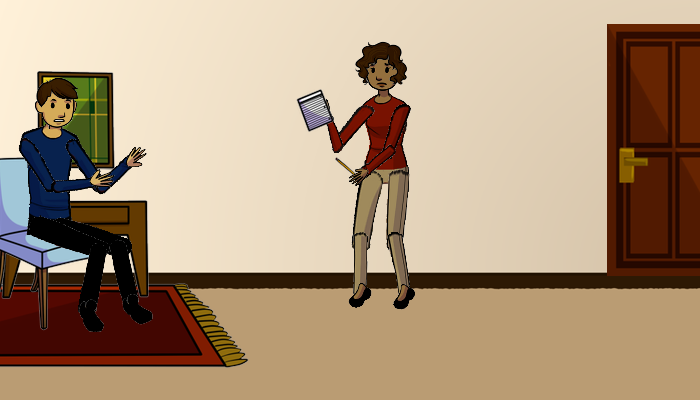
\includegraphics[width=1\linewidth]{image0}
  \caption{\textbf{Q}: Is the man's shirt blue? \textbf{A}: Yes}
  \label{fig:sub1}
\end{subfigure}\
\end{figure}

\section{Dataset}
The dataset is composed by 29333 total images, 58832 training questions and 6372 test questions.


	\subsection{Images}
The images' properties are:
\begin{itemize}
\item{color space: RGB;}
\item{image size: 400x700 pixels;}
\item{file format: png;}
\end{itemize}
	\subsection{Answers}
The set of the possible answers is static and made of 58 possible answers belonging to 3 possible categories: 'yes/no' answers, 'counting' answers (from 0 to 5) and 'other' (e.g., colors, objects, ecc.). In the following the labels associated to each answer:

	\subsection{Data augmentation}
We have not performed data augmentation. The dataset dimension was big enough for the complexity of our model and performing augmentation would have required a lot of time to adapt all the question/answer couples. Furthermore, we could do it just on the images and not on the answers set.
	\section{Validation set}

No automatic validation set is provided. This means that a subset of the training set must be used to perform validation.

In our case, we parametrized the number of training images to be moved into the validation set, with a 10\% probability.


	\section{Test set}
The test set is provided as a set of 6372 (image-question) couples, without the attached answers. Participants are required to provide the answers for the test images by submitting the solution with the correct submission format.

	\section{Evaluation}
Submissions are evaluated on Multiclass Accuracy, which is simply the average number of observations with the correct label.

	%end of first chapter

	\chapter{Neural network architecture}		
		\section{VGG + LSTM + FFNN}
At first, we have thought about a network that analyzes in parallel the image and the question, using
\begin{itemize}
\item{a convolutional network to extract the features from the images;}
\item{an LSTM to process the question and extract the hidden state.}
\end{itemize}
The two results are merged using a multiplication layer and then they are fed to the feed-forward neural network.
A GAP layer is used after the CNN to adapt the output shape to the one of the LSTM.
\begin{figure}[H]
\renewcommand*\thesubfigure{\arabic{subfigure}} 
\centering
\begin{subfigure}{\textwidth}
  \centering
  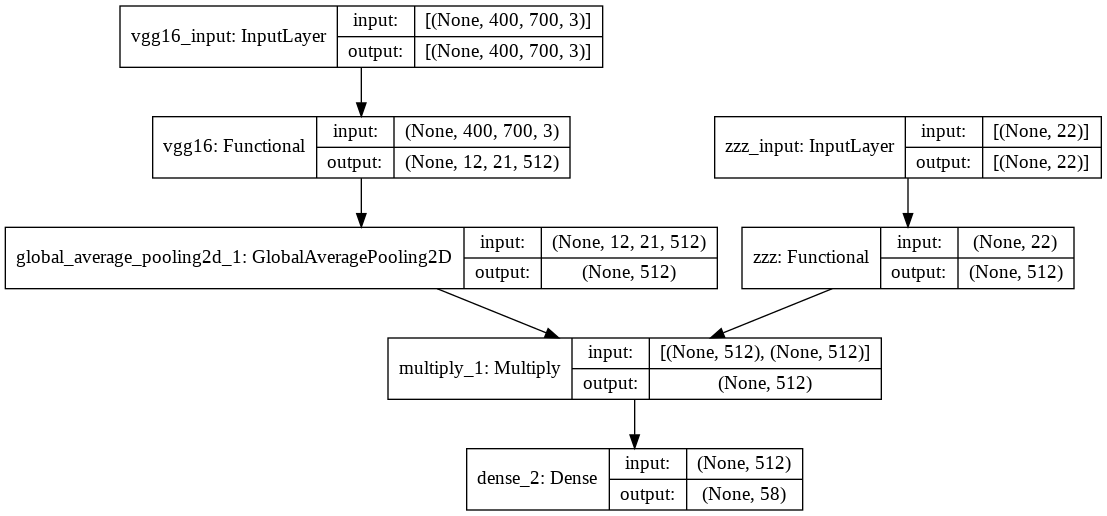
\includegraphics[width=1\linewidth]{model}
  \caption{network architecture}
  \label{fig:sub1}
\end{subfigure}
\end{figure}
\subsection{Score}
	The best score of the network was 0.66211, obtained with the following settings:

\begin{itemize}
	\item VGG standard preprocessing;
	\item \texttt{freeze\_until} = 17;
	\item learning rate = 5e-4;
	\item 10\% validation.
\end{itemize}
		
	%end of second chapter

\chapter{Model tuning}
Our first network had a bidirectional LSTM and one more hidden layer in the FFNN. We were fine-tuning VGG deeply, but we noticed that the model overfitted rapidly. We thought that adding a dropout layer in the FFNN could be a good idea to avoid that behaviour, but the model kept overfitting after few epochs.
 So we decided to reduce the model complexity, by removing the hidden layer in the FFNN, moving to a uni-directional LSTM and freezing more layers of VGG.

Then, we tried to replace VGG with InceptionResNetV2, as it provided better performance in the previous challenges, but in this case, it turned out to be slightly worst than VGG.

Since we obtained pretty good results straight from the first tries, we decided not to drastically change the architecture of the network.
	%end of third chapter
	\chapter{References}
		\section{Links}

\begin{itemize}
	\item GitHub repository of the project: \url{https://github.com/tizianofucci/A2NDLVisualQuestionAnswering}
	\item Competition web page: \url{https://www.kaggle.com/c/anndl-2020-vqa}
\end{itemize}

\end{document}
